% Part: sets-functions-relations
% Chapter: relations
% Section: graphs

\documentclass[../../../include/open-logic-section]{subfiles}

\begin{document}

\olfileid[fr]{sfr}{rel}{grp}
\olsection{Graphes}

Un \emph{graphe} se représente par un diagramme dans lequel des points,
appelés « nœuds » ou « sommets », sont reliés par des arêtes.
Les graphes sont omniprésents en mathématiques discrètes et en informatique.
Ils sont très utiles pour représenter et visualiser des relations et
des structures, qu’il s’agisse d’objets concrets, comme divers réseaux,
ou de structures abstraites, comme les issues possibles d’une décision.
La littérature étudie de nombreux types de graphes : les arêtes peuvent
être orientées ou non, porter ou non des étiquettes ; on peut autoriser
ou interdire une arête reliant un nœud à lui-même, plusieurs arêtes entre
les mêmes nœuds, etc. Les \emph{graphes orientés} entretiennent un lien
particulier avec les relations.

\begin{defn}[Graphe orienté]
Un \emph{graphe orienté} $G = \tuple{V, E}$ est constitué d’un ensemble
de \emph{sommets}~$V$ et d’un ensemble d’\emph{arêtes}~$E \subseteq V^2$.
\end{defn}

\begin{explain}
Selon notre définition, un graphe est simplement un ensemble muni d’une
relation sur cet ensemble. Il est bien sûr naturel d’en attendre une
représentation graphique : on peut le dessiner en traçant une flèche du
sommet~$v_1$ vers le sommet $v_2$ si et seulement si
$\tuple{v_1, v_2} \in E$. La seule différence entre une relation considérée
en elle-même et un graphe est que le graphe précise l’ensemble des sommets ;
il peut donc comporter des sommets isolés. Le point essentiel est que
toute relation~$R$ sur un ensemble~$X$ peut être considérée comme un graphe
orienté $\tuple{X, R}$ et que, réciproquement, un graphe
orienté~$\tuple{V, E}$ peut être considéré comme une relation
$E \subseteq V^2$ dont l’ensemble $V$ est explicitement indiqué.
\end{explain}

\begin{ex}
Le graphe $\tuple{V, E}$ défini par $V = \{1, 2, 3, 4\}$ et
$E = \{\tuple{1,1}, \allowbreak \tuple{1, 2}, \allowbreak \tuple{1, 3},
\allowbreak \tuple{2, 3}\}$ se représente ainsi :
\begin{align*}
& 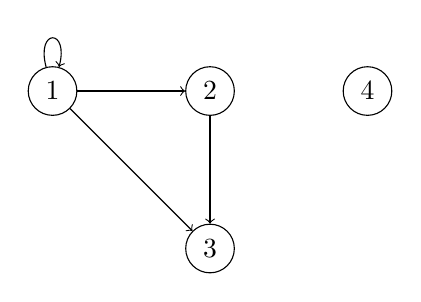
\begin{tikzpicture}[->,node distance=2cm]
  \node[draw,circle] (A) {$1$};
  \node[draw,circle] (B) [right of=A] {$2$};
  \node[draw,circle] (C) [below of=B] {$3$};
  \node[draw,circle] (D) [right of=B] {$4$};
  \draw (A) to [loop above]  (A);
  \draw (A) to  (B);
  \draw (A) to  (C);
  \draw (B) to  (C);
  \end{tikzpicture}
\intertext{Il diffère du graphe $\tuple{V', E}$ où
  $V' = \{1, 2, 3\}$, représenté ci-dessous :}
& 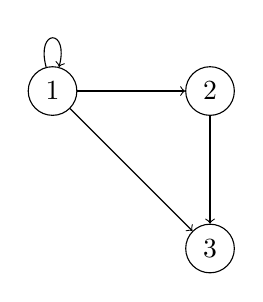
\begin{tikzpicture}[->,node distance=2cm]
  \node[draw,circle] (A) {$1$};
  \node[draw,circle] (B) [right of=A] {$2$};
  \node[draw,circle] (C) [below of=B] {$3$};
  \draw (A) to [loop above]  (A);
  \draw (A) to  (B);
  \draw (A) to  (C);
  \draw (B) to  (C);
  \end{tikzpicture}
\end{align*}
\end{ex}

\begin{prob}
Considérez la relation « inférieur ou égal à »~$\le$ sur l’ensemble
$\{1, 2, 3, 4\}$ comme un graphe et dessinez le diagramme correspondant.
\end{prob}

\end{document}
